\documentclass{article}
\usepackage[utf8]{inputenc}
\usepackage[spanish]{babel}
\usepackage[]{amsthm}
\usepackage{amsmath}
\usepackage[]{amssymb}
\usepackage{graphicx}
\usepackage{wrapfig}
\usepackage[letterpaper, margin=1.5in]{geometry}
\usepackage[hidelinks]{hyperref}
\decimalpoint

\begin{document}
    \begin{titlepage}
        \begin{center}
            \begin{figure}
                \centering
                \includegraphics[scale=0.13]{img/logo_itesm.png}\\ % Logo de la institución
            \end{figure}
        \vspace{5cm}
        \LARGE{Instituto Tecnológico y de Estudios Superiores de Monterrey}\\
        \fontsize{12}{14}\selectfont
        \vspace{1cm}
        \textbf{Tarea 2 Evaluada}\\ % Nombre de la tarea
        \vspace{0.7cm}
        \begin{table}[h!]
            \centering
            \begin{tabular}{ ||c|c|| }
                \hline
                Nombre & Matrícula \\
                \hline
                Juan Pablo Echeagaray González & A00830646 \\
                \hline
                Verónica Victoria García De la Fuente & A00830383 \\
                \hline
                Emily Rebeca Méndez Cruz & A00830768 \\
                \hline
                Eugenio Santiesteban Zolezzi & A01720932 \\
                \hline
                Daniel de Zamacona Madero & A01570576 \\
                \hline
            \end{tabular}
        \end{table}
        \vspace{0.7cm}
        Optimización Estocástica\\ % Materia
        \vspace{0.2cm}
        MA2004B\\ % Clave de la materia
        \vspace{0.2cm}
        Jaime Eduardo Martínez Sánchez\\ % Nombre del profesor
        \vspace{0.7cm}
        15 de agosto del 2022\\ % Fecha de entrega
        \end{center}
    \end{titlepage}

    \section*{Problemas}

        \subsection*{Problema 1}
            Use una ruleta con 6 colores diferentes y equi-probables, y simule la probabilidad de éxito de cada una de ellas. Realice 100 réplicas.

            El resultado de esta simulación puede observarse en la figura \ref{fig:simulacion-ruleta-1}.

            \begin{figure}[!htbp]
                \centering
                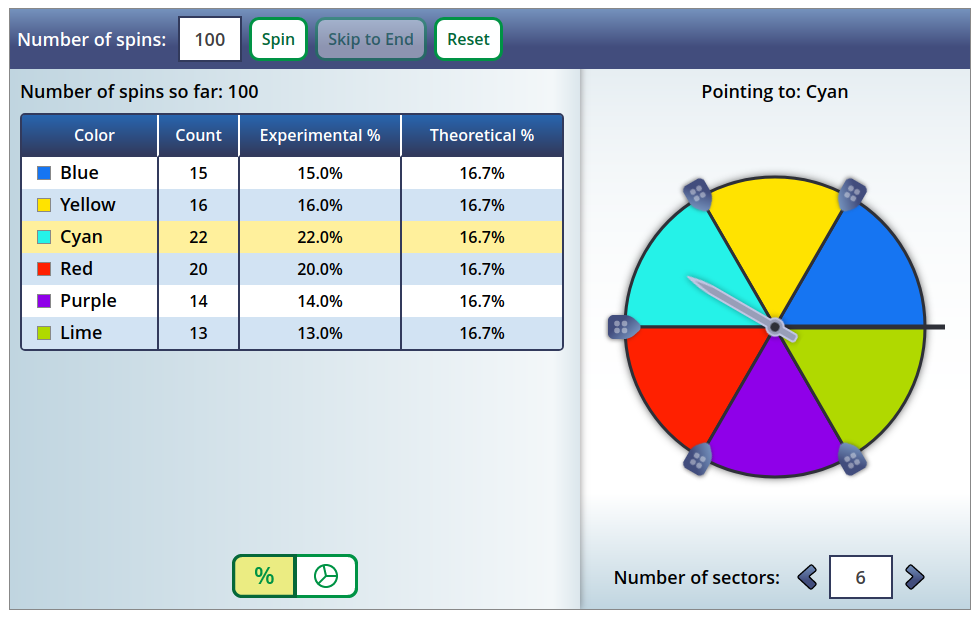
\includegraphics[scale=0.3]{img/simulacion-ruleta-1.png}
                \caption{Simulación de la ruleta con 6 colores diferentes y equi-probables}
                \label{fig:simulacion-ruleta-1}
            \end{figure}

        \subsection*{Problema 2}

            Use 4 colores diferentes en la ruleta, de tal forma que el primer color tenga el doble de probabilidad de éxito del segundo color, el segundo color tenga la tercera parte de probabilidad del tercer color, y el último color tenga una probabilidad de éxito igual a la mitad de la suma de las probabilidades del segundo y tercer color.
            
            \begin{enumerate}
                \item Calcule la probabilidad teórica de éxito de cada color.
                \item Use la ruleta para simular las probabilidades del inciso anterior usando 200 réplicas
            \end{enumerate}

            En este caso, el calcular la probabilidad teórica de éxito de cada uno de los colores se traduce en resolver un sistema de ecuaciones lineales; esto porque del problema sabemos lo siguiente:
            \begin{gather*}
                \sum_{i=1}^{4} P(x_i) = 1 \\
                P(x_1) = 2 P(x_2) \\
                P(x_2) = \frac{1}{3} P(x_3) \\
                P(x_4) = \frac{1}{2} (P(x_2) + P(x_3))
            \end{gather*}

            Si ahora traducimos este sistema de ecuaciones que tiene como variables probabilidades a uno en el que solamente se trabajen con simples variables, tenemos:
            \begin{gather*}
                x_1 + x_2 + x_3 + x_4 = 1 \\
                x_1 - 2x_2 = 0 \\
                x_2 - \frac{1}{3}x_3 = 0 \\
                -\frac{1}{2}x_2 - \frac{1}{2}x_3 + x_4 = 0
            \end{gather*}

            Cuando resolvemos este sistema de ecuaciones llegamos al siguiente vector de probabilidades:
            \begin{equation*}
                \vec{P} = \begin{bmatrix}
                    0.25 \\
                    0.125 \\
                    0.375 \\
                    0.25
                \end{bmatrix}
            \end{equation*}

            Así, la probabilidad de cada color es respectivamente cada una de las entradas del vector anterior. Simulando esto con la ruleta de colores, observamos las probabilidades experimentales en la figura \ref{fig:simulacion-ruleta-2}:

            \begin{figure}[!htbp]
                \centering
                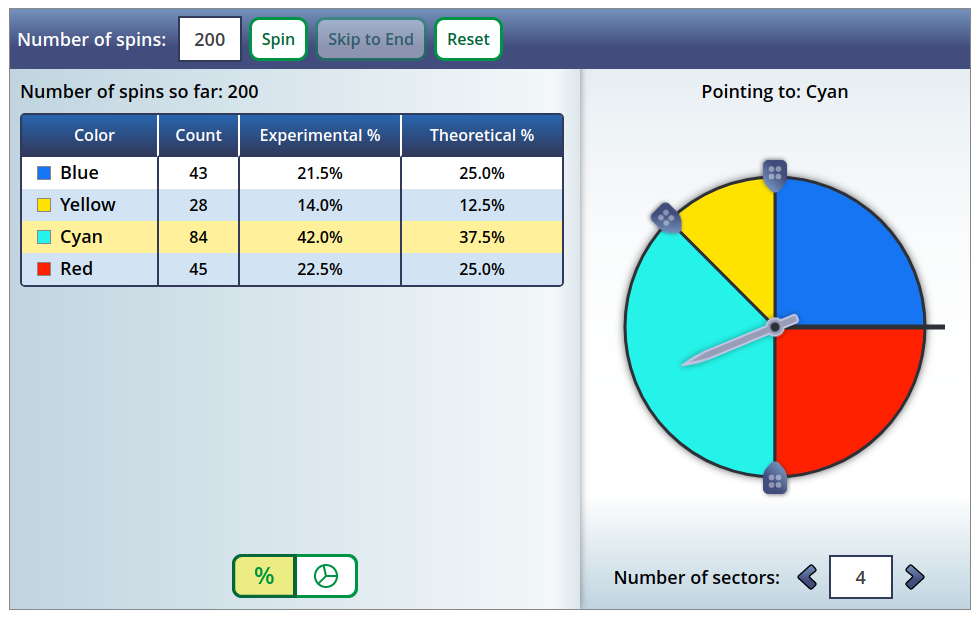
\includegraphics[scale=0.3]{img/simulacion-ruleta-2.png}
                \caption{Simulación de la ruleta con 4 colores diferentes y probabilidades distintas}
                \label{fig:simulacion-ruleta-2}
            \end{figure}

        \subsection*{Problema 3}

            Una agencia distribuidora de autos, tiene disponible en exhibición para su venta los siguientes productos: 15 coches compactos, 5 coches de lujo, 8 camionetas y 7 jeeps. Un hotel va a realizar una compra de 5 unidades, la agencia está interesada en conocer la probabilidad de que el hotel compre 2 coches de lujo y 3 camionetas.

            \begin{enumerate}
                \item Encuentre la probabilidad teórica de este evento.
                \item Use la ruleta para simular la probabilidad el inciso anterior.
                \item Realizar un código (en R, Matlab, Python, etc.) para simular el resultado del inciso 1.
            \end{enumerate}
        
            Reconociendo que la distribución que seguirá este experimento es de carácter hipergeométrico multivariado, podemos calcular la probabilidad teórica solicitada mediante la ecuación:

            \begin{gather*}
                P(0, 2, 3, 0) = \frac{\binom{15}{0} \binom{5}{2} \binom{8}{3} \binom{7}{0}}{\binom{35}{5}} \\
                P(0, 2, 3, 0) \simeq 0.017
            \end{gather*}

        \subsection*{Problema 4}

            En una urna se tienen 30 canicas rojas, 24 negras, 8 amarillas, 15 blancas y 13 verdes. Si se procede a sacar aleatoriamente 5 canicas sin reemplazo y nos interesa obtener la probabilidad de que 2 canicas sean del mismo color, 
            \begin{enumerate}
                \item Calcule la probabilidad exacta de este evento.
                \item Realice una simulación de 50 réplicas para obtener una estimación de la probabilidad solicitada en el inciso anterior
            \end{enumerate}

        \subsection*{Problema 5}

            Una cadena de Markov, $\{X_t\}_{t=1}^{\infty}$, con 3 estados tiene la siguiente matriz de transición:
            \begin{equation*}
                \mathbf{P} = \begin{bmatrix}
                    \frac{1}{3} & \frac{1}{2} & \frac{1}{6} \\[6pt]
                    \frac{1}{4} & \frac{11}{20} & \frac{1}{5} \\[6pt]
                    \frac{1}{5} & \frac{3}{5} & \frac{1}{5}
                \end{bmatrix}
            \end{equation*}

            Calcule las siguientes probabilidades:
            \begin{enumerate}
                \item $\mathbb{P}(X_2 = 0 \mid X_0 = 1)$
                \item $\mathbb{P}(X_3 = 2 \mid X_0 = 2)$
                \item $\mathbb{P}(X_2 = 1)$
                \item $\mathbb{P}(X_2 = 1 \mid X_0 = 1)$
                \item $\mathbb{P}(X_3 = 2 \mid X_0 = 1)$
                \item $\mathbb{P}(X_3 = 0)$
            \end{enumerate}
            
            Para el inciso 1:
            \begin{gather*}
                \mathbb{P}(X_2 = 0 \mid X_0 = 1) = P_{10} P_{00} + P_{11} P_{10} + P_{12} P_{20} \\
                \mathbb{P}(X_2 = 0 \mid X_0 = 1) = \frac{1}{4} \cdot \frac{1}{3} + \frac{11}{20} \cdot \frac{1}{4} + \frac{1}{5} \cdot \frac{1}{5} \\
                \mathbb{P}(X_2 = 0 \mid X_0 = 1) = \frac{313}{1200} \simeq 0.26083
            \end{gather*}
            
            Para el inciso 2:
            \begin{equation*}
                \begin{split}
                    \mathbb{P}(X_3 = 2 \mid X_0 = 2) = & P_{22} P_{22} P_{22} + P_{20} P_{02} P_{22} + P_{20} P_{00} P_{02} + P_{22} P_{20} P_{02} + P_{21}P_{12}P_{22} + \\ & P_{21} P_{11} P_{22} + P_{22}P_{21}P_{12} + P_{20}P_{01}P_{12} + P_{21}P_{10}P_{02} \\
                    \mathbb{P}(X_3 = 2 \mid X_0 = 2) = & \frac{1}{5} \cdot \frac{1}{5} \cdot \frac{1}{5} + \frac{1}{5} \cdot \frac{1}{6} \cdot \frac{1}{5} + \frac{1}{5} \cdot \frac{1}{3} \cdot \frac{1}{6} + \frac{1}{5} \cdot \frac{1}{5} \cdot \frac{1}{6} + \frac{3}{5} \cdot \frac{1}{5} \cdot \frac{1}{5} \\ & + \frac{3}{5} \cdot \frac{11}{20} \cdot \frac{1}{5} + \frac{1}{5} \cdot \frac{3}{5} \cdot \frac{1}{5} + \frac{1}{5} \cdot \frac{1}{2} \cdot \frac{1}{5} + \frac{3}{5} \cdot \frac{1}{4} \cdot \frac{1}{6} \\
                    \mathbb{P}(X_3 = & 2 \mid X_0 = 2) = \frac{1723}{9000} \simeq 0.19144
                \end{split}
            \end{equation*}

            Para el inciso 3 no se dispone de un vector de probabilidades para los estados iniciales, así que supondremos que los 3 estados tienen la misma probabilidad de haber ocurrido:
            \begin{equation*}
                \begin{split}
                    \mathbb{P}(X_2 = 1) &= \mathbb{P}(X_2 = 1 \mid X_0 = 0) \mathbb{P}(X_0 = 0) + \mathbb{P}(X_2 = 1 \mid X_0 = 1) \mathbb{P}(X_0 = 1) + \\ & \mathbb{P}(X_2 = 1 \mid X_0 = 2) \mathbb{P}(X_0 = 2)
                \end{split}
            \end{equation*}

            \begin{gather*}
                \mathbb{P}(X_2 = 1 \mid X_0 = 0) = P_{00} P_{01} + P_{01} P_{11} + P_{02} P_{21} \\
                \mathbb{P}(X_2 = 1 \mid X_0 = 0) = \frac{1}{3} \cdot \frac{1}{2} + \frac{1}{2} \cdot \frac{11}{20} + \frac{1}{6} \cdot \frac{3}{5} \\
                \mathbb{P}(X_2 = 1 \mid X_0 = 0) = \frac{13}{24} \\
                \mathbb{P}(X_2 = 1 \mid X_0 = 1) = P_{11} P_{11} + P_{10} P_{01} + P_{12} P_{21} \\
                \mathbb{P}(X_2 = 1 \mid X_0 = 1) = \frac{11}{20} \cdot \frac{11}{20} + \frac{1}{4} \cdot \frac{1}{2} + \frac{1}{5} \cdot \frac{3}{5} \\
                \mathbb{P}(X_2 = 1 \mid X_0 = 1) = \frac{219}{400} \\
                \mathbb{P}(X_2 = 1 \mid X_0 = 2) = P_{21} P_{11} + P_{22} P_{21} + P_{20} P_{01} \\
                \mathbb{P}(X_2 = 1 \mid X_0 = 2) = \frac{3}{5} \cdot \frac{11}{20} + \frac{1}{5} \cdot \frac{3}{5} + \frac{1}{5} \cdot \frac{1}{2} \\
                \mathbb{P}(X_2 = 1 \mid X_0 = 2) = \frac{11}{20} \\
                \mathbb{P}(X_2 = 1) = \frac{1}{3} \left(\frac{13}{24} + \frac{219}{400} + \frac{11}{20}\right) \\
                \mathbb{P}(X_2 = 1) = \frac{1967}{3000} \simeq 0.54638
            \end{gather*}

            Para el inciso 4:
            \begin{equation*}
                \mathbb{P}(X_2 = 1 \mid X_0 = 0) = P_{00} P_{01} + P_{01} P_{11} + P_{02} P_{21} = \frac{13}{24}
            \end{equation*}

            Para el inciso 5:
            \begin{equation*}
                \begin{split}
                    \mathbb{P}(X_3 = 2 \mid X_0 = 1) = & P_{12} P_{22} P_{22} + P_{10} P_{01} P_{12} + P_{12} P_{21} P_{22} +P_{11} P_{11} P_{12} + \\ & P_{10} P_{00} P_{02} + P_{12} P_{20} P_{02} + P_{11} P_{12} P_{22} + P_{11} P_{10} P_{02} + P_{10} P_{02} P_{22} \\
                    \mathbb{P}(X_3 = 2 \mid X_0 = 1) = & \frac{1}{5} \cdot \frac{1}{5} \cdot \frac{1}{5} + \frac{1}{4} \cdot \frac{1}{2} \cdot \frac{1}{5} + \frac{1}{5} \cdot \frac{3}{5} \cdot \frac{1}{5} + \frac{11}{20} \cdot \frac{11}{20} \cdot \frac{1}{5} + \frac{1}{4} \cdot \frac{1}{3} \cdot \frac{1}{6} + \\ &\frac{1}{5} \cdot \frac{1}{5} \cdot \frac{1}{6} + \frac{11}{20} \cdot \frac{1}{5} \cdot \frac{1}{5} + \frac{11}{20} \cdot \frac{1}{4} \cdot \frac{1}{6} + \frac{1}{4} \cdot \frac{1}{6} \cdot \frac{1}{5} \\
                    \mathbb{P}(X_3 = 2 \mid X_0 = 1) = & \frac{6887}{36000} \simeq 0.1913055
                \end{split}
            \end{equation*}

            Para el inciso 6 se aplica la misma lógica que en el inciso 3, no disponemos de un vector de probabilidades iniciales para cada uno de los estados, por lo que supondremos que cada uno tuvo la misma probabilidad de haber ocurrido:
            \begin{equation*}
                \begin{split}
                    \mathbb{P}(X_3 = 0) &= \mathbb{P}(X_3 = 0 \mid X_0 = 0) \mathbb{P}(X_0 = 0) + \mathbb{P}(X_3 = 0 \mid X_0 = 1) \mathbb{P}(X_0 = 1) + \\ & \mathbb{P}(X_3 = 0 \mid X_0 = 2) \mathbb{P}(X_0 = 2)
                \end{split}
            \end{equation*}
            
            \begin{equation*}
                \begin{split}
                    \mathbb{P}(X_3 = 0 \mid X_0 = 0) =& P_{00} P_{00} P_{00} +  P_{01} P_{11} P_{10} +  P_{02} P_{22} P_{20} + P_{01} P_{12} P_{20} + P_{02} P_{21} P_{10} + \\ & P_{00} P_{01} P_{10} + P_{00} P_{02} P_{20} + P_{01} P_{10} P_{00} + P_{02} P_{20} P_{00} \\
                    \mathbb{P}(X_3 = 0 \mid X_0 = 0) =& \frac{5681}{21600} \simeq 0.263 \\
                    \mathbb{P}(X_3 = 0 \mid X_0 = 1) =& P_{11} P_{11} P_{10} + P_{10} P_{00} P_{00} + P_{11} P_{10} P_{00} + P_{12} P_{21} P_{10} + P_{12} P_{22} P_{20} + \\ & P_{11} P_{12} P_{20} + P_{10} P_{01} P_{10} + P_{10} P_{02} P_{20} + P_{12} P_{20} P_{00}\\
                    \mathbb{P}(X_3 = 0 \mid X_0 = 1) =& \frac{151}{576} \simeq 0.262 \\
                    \mathbb{P}(X_3 = 0 \mid X_0 = 2) =& P_{22} P_{22} P_{20} + P_{22} P_{20} P_{00} + P_{22} P_{21} P_{10} + P_{20} P_{00} P_{00} + P_{20} P_{02} P_{20} + \\ & P_{20} P_{01} P_{10} + P_{21} P_{10} P_{00} + P_{21} P_{12} P_{20} + P_{21} P_{11} P_{10} \\
                    \mathbb{P}(X_3 = 0 \mid X_0 = 2) =& \frac{4711}{18000} \simeq 0.26172 \\
                    \mathbb{P}(X_3 = 0) =& \frac{1}{3} \left(\frac{5681}{21600} + \frac{151}{576} + \frac{4711}{18000}\right) = \frac{169967}{648000} \simeq 0.262294
                \end{split}
            \end{equation*}
        \clearpage
        \appendix
        
        \section{Código desarrollado}
                
\end{document}